
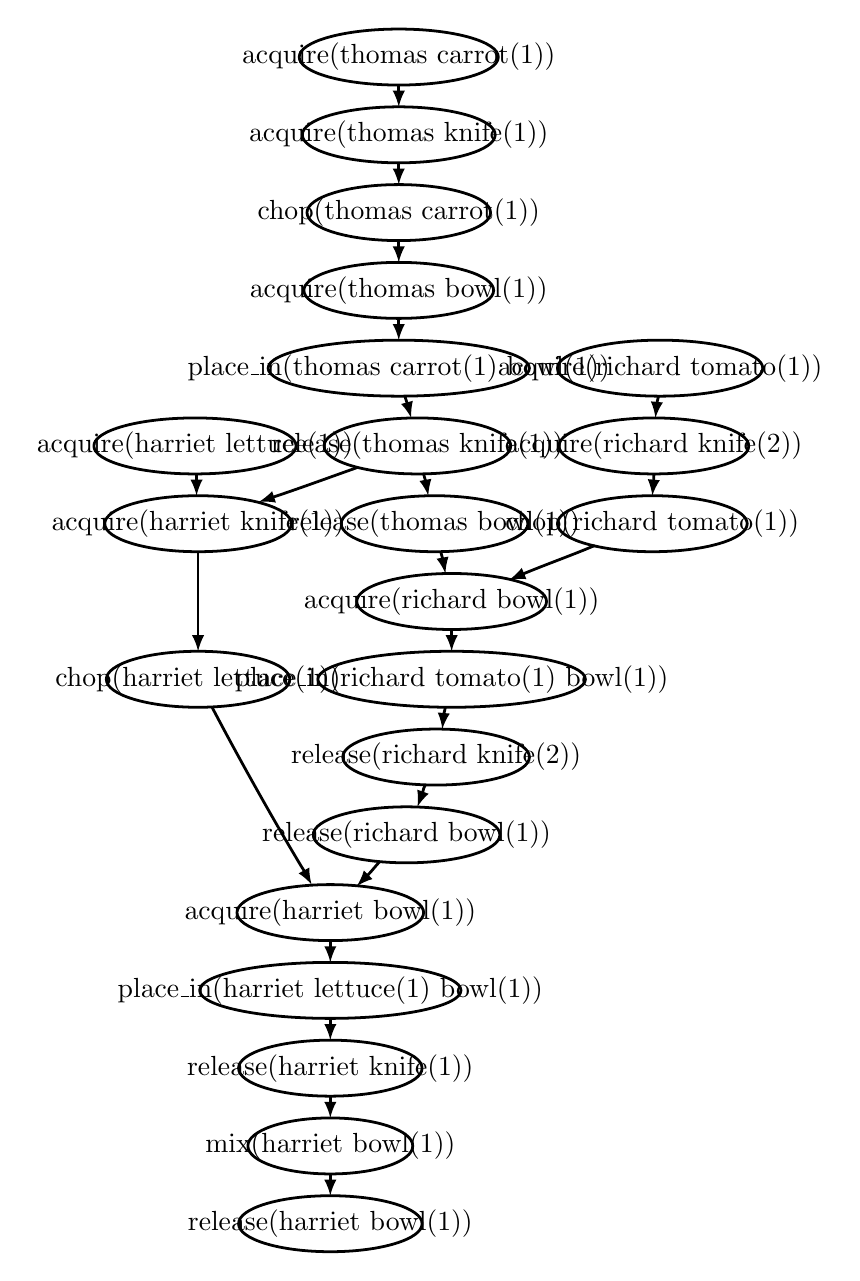
\begin{tikzpicture}[>=latex,join=bevel,scale=0.56]
  \pgfsetlinewidth{1bp}
%
\pgfsetcolor{black}
  % Edge: n0 -> n6
  \draw [->] (196bp,750bp) .. controls (196bp,749bp) and (196bp,748bp)  .. (196bp,736bp);
  % Edge: n2 -> n8
  \draw [->] (363bp,550bp) .. controls (363bp,549bp) and (362bp,547bp)  .. (361bp,536bp);
  % Edge: n6 -> n10
  \draw [->] (196bp,700bp) .. controls (196bp,699bp) and (196bp,698bp)  .. (196bp,686bp);
  % Edge: n8 -> n12
  \draw [->] (360bp,500bp) .. controls (360bp,499bp) and (360bp,497bp)  .. (359bp,486bp);
  % Edge: n10 -> n14
  \draw [->] (196bp,650bp) .. controls (196bp,649bp) and (196bp,648bp)  .. (196bp,636bp);
  % Edge: n14 -> n16
  \draw [->] (196bp,600bp) .. controls (196bp,599bp) and (196bp,598bp)  .. (196bp,586bp);
  % Edge: n16 -> n18
  \draw [->] (200bp,550bp) .. controls (200bp,549bp) and (201bp,547bp)  .. (204bp,536bp);
  % Edge: n18 -> n20
  \draw [->] (212bp,500bp) .. controls (212bp,499bp) and (213bp,497bp)  .. (215bp,486bp);
  % Edge: n18 -> n22
  \draw [->] (169bp,504bp) .. controls (152bp,498bp) and (133bp,491bp)  .. (106bp,482bp);
  % Edge: n4 -> n22
  \draw [->] (66bp,500bp) .. controls (66bp,499bp) and (66bp,498bp)  .. (66bp,486bp);
  % Edge: n20 -> n24
  \draw [->] (223bp,450bp) .. controls (223bp,449bp) and (224bp,447bp)  .. (226bp,436bp);
  % Edge: n12 -> n24
  \draw [->] (322bp,454bp) .. controls (308bp,448bp) and (291bp,442bp)  .. (267bp,432bp);
  % Edge: n22 -> n26
  \draw [->] (67bp,450bp) .. controls (67bp,435bp) and (67bp,413bp)  .. (67bp,386bp);
  % Edge: n24 -> n28
  \draw [->] (230bp,400bp) .. controls (230bp,399bp) and (230bp,398bp)  .. (230bp,386bp);
  % Edge: n28 -> n30
  \draw [->] (226bp,350bp) .. controls (226bp,349bp) and (225bp,347bp)  .. (224bp,336bp);
  % Edge: n30 -> n32
  \draw [->] (213bp,300bp) .. controls (212bp,299bp) and (212bp,297bp)  .. (208bp,286bp);
  % Edge: n32 -> n34
  \draw [->] (184bp,251bp) .. controls (181bp,248bp) and (179bp,245bp)  .. (169bp,235bp);
  % Edge: n26 -> n34
  \draw [->] (76bp,350bp) .. controls (88bp,327bp) and (111bp,285bp)  .. (132bp,250bp) .. controls (133bp,248bp) and (134bp,247bp)  .. (140bp,236bp);
  % Edge: n34 -> n36
  \draw [->] (152bp,200bp) .. controls (152bp,199bp) and (152bp,198bp)  .. (152bp,186bp);
  % Edge: n36 -> n38
  \draw [->] (152bp,150bp) .. controls (152bp,149bp) and (152bp,148bp)  .. (152bp,136bp);
  % Edge: n38 -> n40
  \draw [->] (152bp,100bp) .. controls (152bp,99bp) and (152bp,98bp)  .. (152bp,86bp);
  % Edge: n40 -> n42
  \draw [->] (152bp,50bp) .. controls (152bp,49bp) and (152bp,48bp)  .. (152bp,36bp);
  % Node: n0
\begin{scope}
  \pgfsetstrokecolor{black}
  \draw (196bp,768bp) ellipse (64bp and 18bp);
  \draw (196bp,768bp) node {acquire(thomas carrot(1))};
\end{scope}
  % Node: n2
\begin{scope}
  \pgfsetstrokecolor{black}
  \draw (364bp,568bp) ellipse (66bp and 18bp);
  \draw (364bp,568bp) node {acquire(richard tomato(1))};
\end{scope}
  % Node: n4
\begin{scope}
  \pgfsetstrokecolor{black}
  \draw (65bp,518bp) ellipse (65bp and 18bp);
  \draw (65bp,518bp) node {acquire(harriet lettuce(1))};
\end{scope}
  % Node: n6
\begin{scope}
  \pgfsetstrokecolor{black}
  \draw (196bp,718bp) ellipse (62bp and 18bp);
  \draw (196bp,718bp) node {acquire(thomas knife(1))};
\end{scope}
  % Node: n8
\begin{scope}
  \pgfsetstrokecolor{black}
  \draw (360bp,518bp) ellipse (61bp and 18bp);
  \draw (360bp,518bp) node {acquire(richard knife(2))};
\end{scope}
  % Node: n10
\begin{scope}
  \pgfsetstrokecolor{black}
  \draw (196bp,668bp) ellipse (59bp and 18bp);
  \draw (196bp,668bp) node {chop(thomas carrot(1))};
\end{scope}
  % Node: n12
\begin{scope}
  \pgfsetstrokecolor{black}
  \draw (359bp,468bp) ellipse (61bp and 18bp);
  \draw (359bp,468bp) node {chop(richard tomato(1))};
\end{scope}
  % Node: n14
\begin{scope}
  \pgfsetstrokecolor{black}
  \draw (196bp,618bp) ellipse (61bp and 18bp);
  \draw (196bp,618bp) node {acquire(thomas bowl(1))};
\end{scope}
  % Node: n16
\begin{scope}
  \pgfsetstrokecolor{black}
  \draw (196bp,568bp) ellipse (84bp and 18bp);
  \draw (196bp,568bp) node {place\_in(thomas carrot(1) bowl(1))};
\end{scope}
  % Node: n18
\begin{scope}
  \pgfsetstrokecolor{black}
  \draw (208bp,518bp) ellipse (60bp and 18bp);
  \draw (208bp,518bp) node {release(thomas knife(1))};
\end{scope}
  % Node: n20
\begin{scope}
  \pgfsetstrokecolor{black}
  \draw (219bp,468bp) ellipse (60bp and 18bp);
  \draw (219bp,468bp) node {release(thomas bowl(1))};
\end{scope}
  % Node: n22
\begin{scope}
  \pgfsetstrokecolor{black}
  \draw (67bp,468bp) ellipse (60bp and 18bp);
  \draw (67bp,468bp) node {acquire(harriet knife(1))};
\end{scope}
  % Node: n24
\begin{scope}
  \pgfsetstrokecolor{black}
  \draw (230bp,418bp) ellipse (61bp and 18bp);
  \draw (230bp,418bp) node {acquire(richard bowl(1))};
\end{scope}
  % Node: n26
\begin{scope}
  \pgfsetstrokecolor{black}
  \draw (67bp,368bp) ellipse (59bp and 18bp);
  \draw (67bp,368bp) node {chop(harriet lettuce(1))};
\end{scope}
  % Node: n28
\begin{scope}
  \pgfsetstrokecolor{black}
  \draw (230bp,368bp) ellipse (86bp and 18bp);
  \draw (230bp,368bp) node {place\_in(richard tomato(1) bowl(1))};
\end{scope}
  % Node: n30
\begin{scope}
  \pgfsetstrokecolor{black}
  \draw (220bp,318bp) ellipse (60bp and 18bp);
  \draw (220bp,318bp) node {release(richard knife(2))};
\end{scope}
  % Node: n32
\begin{scope}
  \pgfsetstrokecolor{black}
  \draw (201bp,268bp) ellipse (60bp and 18bp);
  \draw (201bp,268bp) node {release(richard bowl(1))};
\end{scope}
  % Node: n34
\begin{scope}
  \pgfsetstrokecolor{black}
  \draw (152bp,218bp) ellipse (60bp and 18bp);
  \draw (152bp,218bp) node {acquire(harriet bowl(1))};
\end{scope}
  % Node: n36
\begin{scope}
  \pgfsetstrokecolor{black}
  \draw (152bp,168bp) ellipse (84bp and 18bp);
  \draw (152bp,168bp) node {place\_in(harriet lettuce(1) bowl(1))};
\end{scope}
  % Node: n38
\begin{scope}
  \pgfsetstrokecolor{black}
  \draw (152bp,118bp) ellipse (59bp and 18bp);
  \draw (152bp,118bp) node {release(harriet knife(1))};
\end{scope}
  % Node: n40
\begin{scope}
  \pgfsetstrokecolor{black}
  \draw (152bp,68bp) ellipse (53bp and 18bp);
  \draw (152bp,68bp) node {mix(harriet bowl(1))};
\end{scope}
  % Node: n42
\begin{scope}
  \pgfsetstrokecolor{black}
  \draw (152bp,18bp) ellipse (59bp and 18bp);
  \draw (152bp,18bp) node {release(harriet bowl(1))};
\end{scope}
%
\end{tikzpicture}

